\documentclass[../main.tex]{subfiles}
\graphicspath{{\subfix{../images/}}}

\begin{document}

\hypertarget{dataset-module}{%
\chapter{The Dataset Module}\label{dataset-module}}

The initial component of the cyber reasoning system is the dataset
module. The aim of this component is to create and manage collections of
vulnerable software programs utilizing public test suites.

An additional prerequisite for the resulting binary files is that they
must be labeled with appropriate information pertaining to their
vulnerabilities. This will aid in calculating the overall system's
accuracy by comparing the vulnerabilities found (correctly or wrongly)
by OpenCRS with the intended ones, as designated in the initial
datasets.

\hypertarget{implementation}{%
\section{Implementation}\label{implementation}}

\hypertarget{embedded-test-suites}{%
\subsection{Embedded Test Suites}\label{embedded-test-suites}}

We began by scanning the public domain for well-known test suites that
had insecure C applications. We filtered out datasets that contained
non-compilable code because OpenCRS analyzes full executables using
static and dynamic analysis techniques. Articles in Academia \cite{c_code_changes_dataset}, for
example, use just the code modifications introduced by a commit, a
property that is incompatible with the executable-level, black-box
analysis done by our CRS. On the other side, we chose to use programs
that had been precisely tagged with vulnerability tags, such as by
constructing synthetic, vulnerable-by-design programs. This contradicts
the strategy of utilizing a static code analyzer (such as SonarCloud \cite{sonarcloud_dataset}) to
find and label potential vulnerabilities in code.

C Test Suite for Source Code Analyzer v2 - Vulnerable \cite{nist_c_test_suite}, developed in
partnership between the National Institute of Standards and Technology
and Alexander Hoole of the University of Victoria in Canada, is one of
the test suites integrated into the dataset modules. It is made up of 54
C source codes plus a manifest file. The latter adheres to the Extensible Markup Language (XML)
standard and includes a \texttt{\textless{}testcase\textgreater{}} entry
for each program in the test suite, as well as the required child tags
listed below. Because each program has a vulnerability, the latter is
stated in each tag on the XPath \texttt{/testcase/file{[}{]}/flaw} and
described in \texttt{line} (i.e.~the line where the security issue
occurs) and \texttt{name} (which is, in fact, the Common Weakness
Enumeration item).

\begin{landscape}
\vspace*{\fill}
\renewcommand*\figurename{Figure}
\begin{figure}[!h]
   \centering
    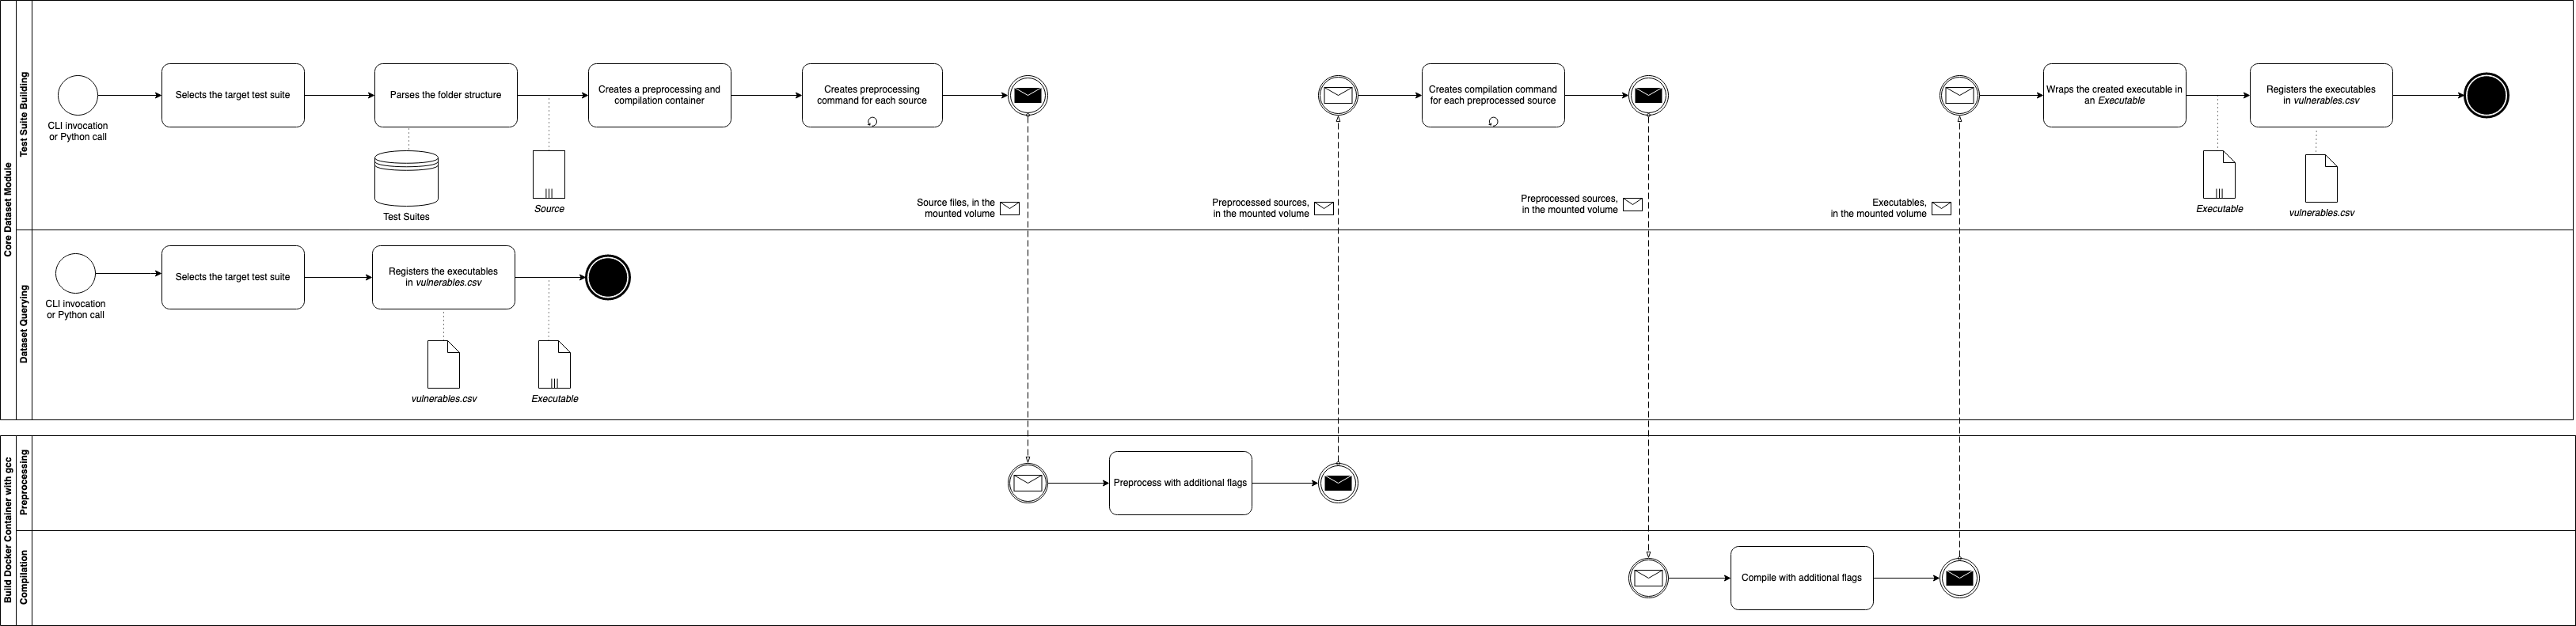
\includegraphics[width=0.95\linewidth]{images/dataset.png}
    \caption{Architecture of the Dataset Module}
    \label{fig:dataset_architecture}
\end{figure}
\vspace*{\fill}
\end{landscape}

Despite the fact that the build command was attached in
\texttt{/testcase/@instruction}, we chose to relocate the build logic
into a separate \texttt{Makefile}. This allows the executable to be
created without first parsing the XML file. We also published this
revision to a separate repository on our GitHub organization \cite{nist_c_test_suite_repo}, in
addition to the test suite. This allowed us to add it to the dataset
repository as a submodule.

The second test suite is Juliet C/C++ 1.3 \cite{nist_juliet}, which is already available on
GitHub \cite{nist_juliet_repo}. The same American institution built it, but in partnership with
the National Security Agency's Center for Assured Software. It consists
of 64123 susceptible test cases and an XML manifest file with minor
variations from the previous one (for example, not having the build
command in \texttt{/testcase/@instruction}).

The necessity for custom binaries became more apparent during the
testing of other components. We ended up building an additional custom
test suite in the dataset module called \texttt{toy\_test\_suite} with a
simple folder structure: a source containing vulnerable code and a
\texttt{cwe.txt} file with the associated Common Weakness Enumeration (CWE) ID. Small executables such
as stack buffer overflows, \texttt{NULL} pointer dereferences, and
tainted format strings were included here.

\hypertarget{test-suites-building.-results-retrieval}{%
\subsection{Test Suites Building. Results
Retrieval}\label{test-suites-building.-results-retrieval}}

These three datasets were linked as submodules in the \texttt{dataset}'s \cite{dataset_module_repo} \texttt{raw\_testsuites} folder. In the
\texttt{dataset.parsers} module, a distinct class (called parser) is
created for each of them. The class should implement the following
abstract methods because it should inherit the \texttt{BaseParser}
class:

\begin{itemize}
\tightlist
\item
  \texttt{\_get\_all\_sources}: Parses \texttt{raw\_testsuites/\textless{}testsuite\_id\textgreater{}}, which is the folder structure of the
  dataset, and returns a list of \texttt{Source} objects. The latter contains
  information such as the full path of the source file and the embedded
  CWEs.
\item
  \texttt{preprocess}: Having the \texttt{Source} objects already
  created, the method deals with preprocessing the sources with
  \texttt{gcc}, eventually by considering custom preprocessing flags.
  The resulting files are placed in the \texttt{sources} folder.
\item
  \texttt{\_generate\_gcc\_command}: Based on the preprocessed sources
  in \texttt{sources} and additional compilation flags, uses
  \texttt{gcc} to compile the executables in \texttt{executables}.
  Further details are placed in a Comma Separated Values (CSV) file, \texttt{vulnerables.csv},
  which has columns indicating the executable ID, the test suite it
  comes from, its CWEs, and a boolean indicating if it is built or not.
\end{itemize}

All \texttt{gcc}-related operations (both preprocessing and building)
are carried out in a Docker container running Ubuntu. This allows for
the replication of the building process as well as separation from the
host operating system. We like to communicate with the container using
volumes (for file sharing) and Docker Application Programmable Interface (API) calls. This was preferable to
using a gRPC service because the module's code resides on the same host
as the build container, and communication delays are reduced by avoiding
transferring large files (e.g.~the sources and executables) via (a
virtualized) network.

A parsers' manager is enabled when the build functionality is started
from the command-line interface or by invoking the specified method from
the Python module. It chooses the necessary parsers and invokes the
preprocessing and construction techniques. The process's output,
specifically \texttt{Executable} objects, can be queried using other
procedures, in which \texttt{vulnerable.csv} is parsed once again.

\end{document}